\pagebreak
\section{Descrizione Design Pattern}
\label{appendice-pattern}

	\subsection{Chain of Responsibility} % patern comportamentale
	Il \glossario{Chain of Responsibility} è un pattern comportamentale che permette di separare i \emph{sender} dai \emph{receiver} delle richieste. La richiesta attraversa una catena di oggetti per essere intercettata solo quando raggiunge il proprio gestore. Viene utilizzato quando non è possibile determinare staticamente il \emph{receiver} oppure l'insieme di oggetti gestori cambia dinamicamente a runtime. \\ Le richieste vengono dette \emph{implicite} poiché il \emph{sender} non ha alcuna conoscenza sull'identità del ricevente. Per permettere alla richiesta di attraversare la catena e per rimanere \emph{implicita}, ogni \emph{receiver} condivide un interfaccia comune per gestire le richieste ed accedere al proprio successore. 
	La gerarchia che vorrà inviare richieste dovrà avere una superclasse che dichiara un metodo \emph{handler} generico, la specializzazione di tale metodo avviene tramite \emph{overriding} nelle sottoclassi opportune, come illustrato in figura \ref{fig:chainofresponsibility}.
	
	\begin{figure}[h]
	\centering 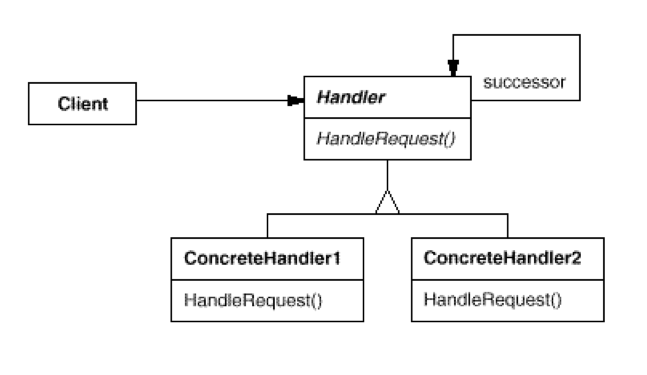
\includegraphics[width=0.7\textwidth]{patterns/ChainOfResponsability.png}
	\caption{Struttura del chain of responsibility.}
	\label{fig:chainofresponsibility}
	\end{figure}
	
	L'utilizzo di questo pattern comporta una serie di conseguenze:
		\begin{itemize}
			\item Ridotto accoppiamento: gli oggetti non sono a conoscenza di chi gestirà la richiesta ma sanno solo che verrà gestita in modo appropriato. Inoltre non bisognerà manutenere i riferimenti a tutti i possibili riceventi;
			\item Aggiunge flessibilità nell'assegnamento delle responsabilità degli oggetti: è possible distribuire le responsabilità tra gli oggetti a runtime modificandone la gerarchia. Staticamente è possibile usare il \emph{subclassing} per specializzare i gestori;
 			\item Non c'è garanzia che la \emph{request} venga gestita, questo può avvenire quando la catena non è stata costruita in modo rigoroso.
		\end{itemize}
	
		
	
	\subsection{Middleware} 
	
	\subsection{Injection} %angular
	
	\subsection{Singleton} % creazionale
	Il \glossario{Singleton} è un design pattern creazionale che permette di avere un unica istanza di una classe con un unico punto di accesso noto. Tale condizione è tipica di alcuni contesti e trova risvolti pratici in svariate applicazioni. Per permettere l'implementazione di questo pattern è sufficiente che la classe stessa si occupi di tracciare la propria istanziazione e bloccarla qualora sia già avvenuta almeno una volta. Il \glossario{Singleton} dovrebbe essere estensibile usando il \emph{subclassing} il client può utilizzarne l'estensione senza quindi modificarne il codice.
	
		\begin{figure}[h]
	\centering 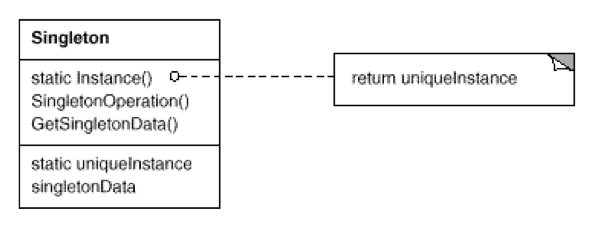
\includegraphics[width=0.7\textwidth]{patterns/Singleton.png}
	\caption{Struttura del singleton.}
	\label{fig:chainofresponsibility}
	\end{figure}
	
	L'utilizzo di questo pattern comporta una serie di conseguenze:
	\begin{itemize}
		\item Accesso controllato alla singola istanza: poiché la classe \glossario{Singleton} incapsula la sua unica istanza, è in grado di controllare quando e come i client vi accedono;
		\item Namespace pulito: l'utilizzo di questo pattern risulta migliore rispetto all'uso di variabili globali poiché scongiura l'inquinamento del name space globale;
		\item Permette raffinamenti di operazioni e rappresentazioni: il \glossario{Singleton} dovrebbe venire sempre esteso prima dell'utilizzo, che in termini pratici si traduce in un operazione banale, questo può avvenire anche in runtime;
		\item Eventualmente permette un numero variabile di istanze: questo pattern permette, se necessario, di avere istanze multiple mantenendo però il controllo sul numero;
		\item Flessibilità; un modo per avere una funzionalità riconducibile al \glossario{Singleton} è quello di utilizzare le operazioni sulle classi, come per esempio la keyword \code{static} del C++, ma in questo modo è più difficile controllarne il design e permetterne più istanze. Inoltre nel linguaggio succitato le funzioni statiche non sono mai virtuali, rendendone impossibile l'utilizzo polimorfo alle sottoclassi che le ridefiniscono.
	\end{itemize}
	
	\subsection{Registry} %libro dropbox